\section{Pipelined Implementation}

For pipelined implementation, a set of stage registers will be placed at every arithmetic operation for memorizing the outcome of every stage.
The required operation \textbf{\(Z = \frac{1}{4} [A^2\ast B] + 1\)} can be divided into three stages of calculation with one overflow handling stage.
Stage 1 should obtain the product of \(A\) and \(A\) and \(B\).
Then stage 2 should perform two bits right shifting operation on the result of stage 1, this operation represents the \(\frac{1}{4}\).
After that, stage 3 will add number 1 to the result of stage 2.
Finally, stage 4 should handle the bit width of the arithmetic result into the required width.

\subsection{8-bit Operands Implementation with Negation Overflow Handling}

By this design, the circuit will obtain the result in 4 synchronized clock cycles after the falling edge event of the \(load\) signal.
\tbref{tb:pip_vi} shows how the registers in this pipelined circuit will latch the values.
\figref{fig:p_8_rtl} presents the RTL description of the circuit and its arithmetic block.

\begin{table}[!ht]
	\renewcommand{\arraystretch}{0.8}
	\caption{A Visual Representation Table of the Pipelined Processing with Negation Overflow Handling}
	\centering
	\begin{tabular}{ >{\centering\arraybackslash}p{0.5cm} >{\centering\arraybackslash}p{1.5cm} >{\centering\arraybackslash}p{2cm} >{\centering\arraybackslash}p{2cm} >{\centering\arraybackslash}p{2cm}>{\centering\arraybackslash}p{2cm} >{\centering\arraybackslash}p{3cm} }
		\hline
		\bfseries clk & \bfseries A Reg & \bfseries B Reg & \bfseries Stage 1 Reg & \bfseries Satge 2 Reg & \bfseries Satge 3 Reg & \bfseries Stage 4 Reg(Z) \\
		\hline
		0             & 12              & 3               & -                     & -                     & -                     & -                        \\
		1             & -               & -               & 432                   & -                     & -                     & -                        \\
		2             & -               & -               & -                     & 108                   & -                     & -                        \\
		3             & -               & -               & -                     & -                     & 109                   & -                        \\
		4             & -               & -               & -                     & -                     & -                     & 109                      \\
		\hline
	\end{tabular}
	\label{tb:pip_vi}
\end{table}

\figref{fig:p_8_sim} shows the simulation wave result of the pipelined ALU circuit.
As can be observed with the figure, once the \(load\) signal goes from 1 to 0, after 4 clock cycles, z obtains the result of the input.
And the circuit is pipelining the data by the falling edge event of \(load\) signal and the \(clock\).
If the \(clk\) signal was asserted, all registers will be reset and \(end\_flag\) turned into 0.

\begin{figure}[!ht]
	\centering
	\caption{Simulation Wave Diagram of the 8-bit Pipelined ALU Circuit with Negation Output}
	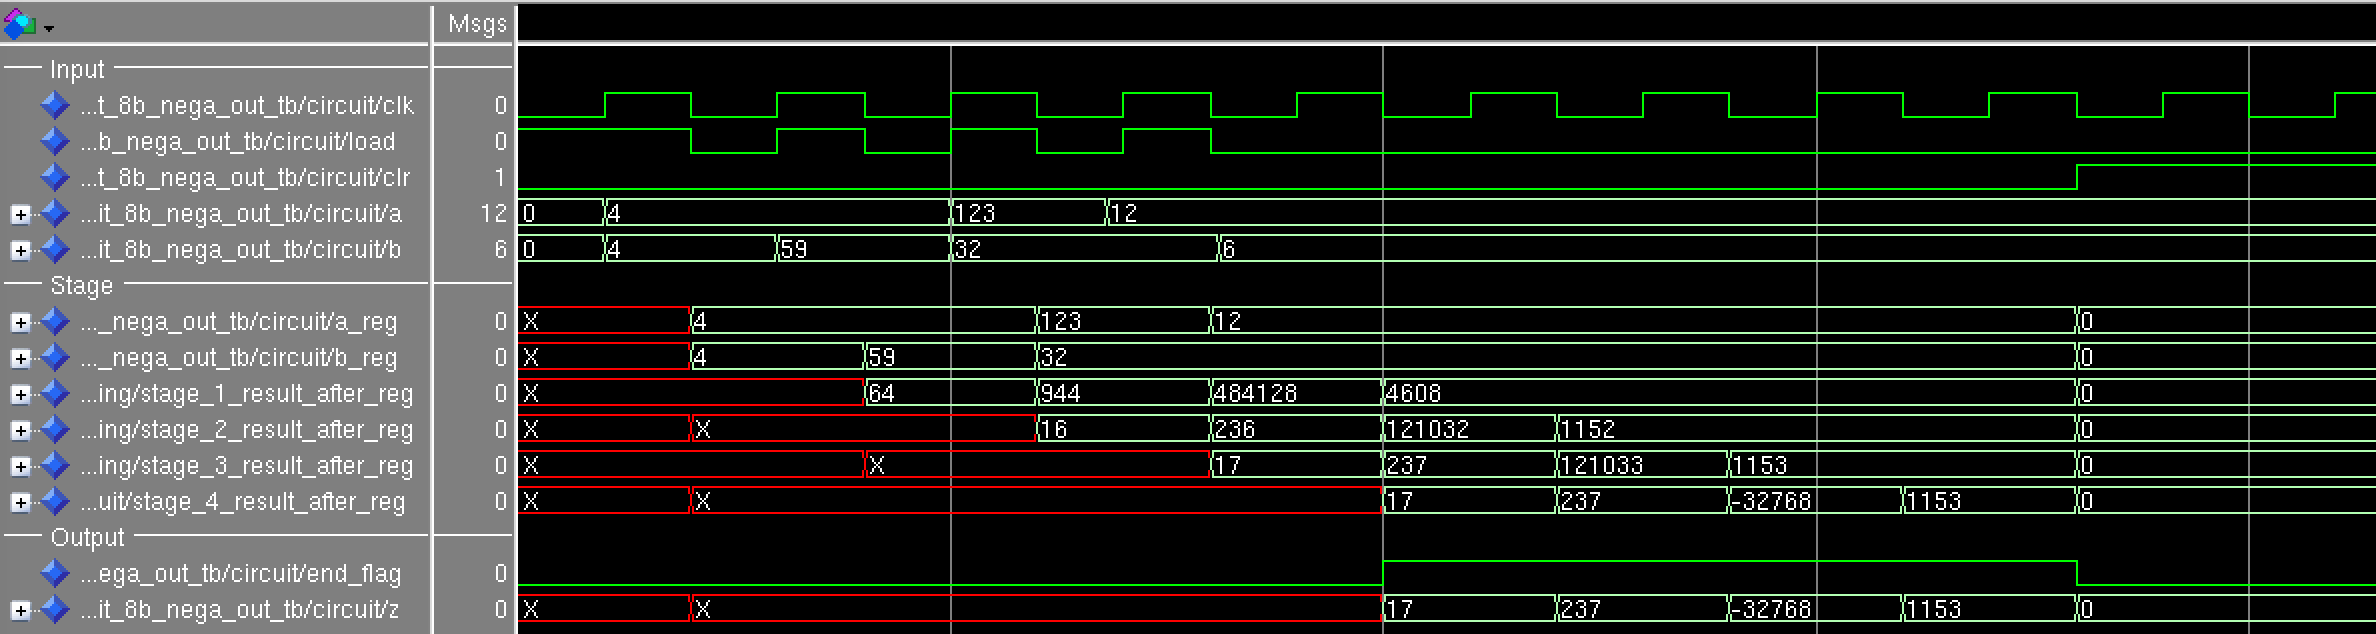
\includegraphics[width=\textwidth]{../img/p_8_sim.png}
	\label{fig:p_8_sim}
\end{figure}

\begin{figure}[!ht]
	\centering
	\caption{Synthesized RTL Diagram of the 8-bit Operands Pipelined ALU Circuit and the Arithmetic Operation Block}

	\subfloat[Top Design of the Circuit]{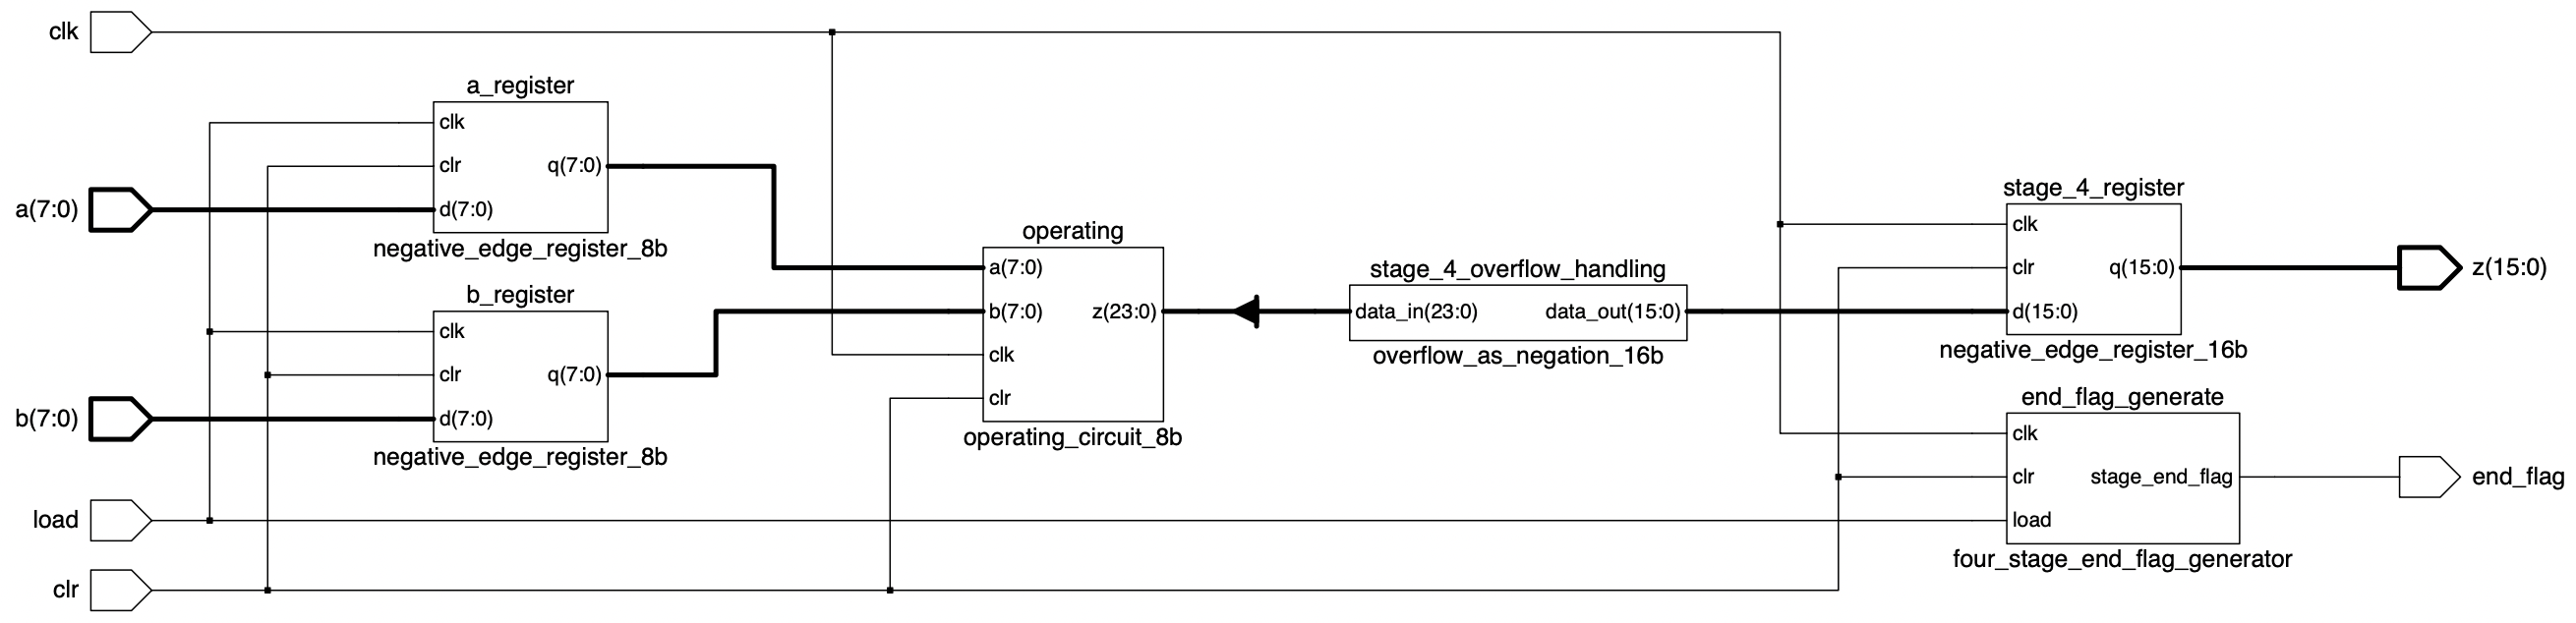
\includegraphics[width=\textwidth]{./img/p_8_rtl.png}}
	\hspace{0.5cm}
	\subfloat[Arithmetic Operation Block]{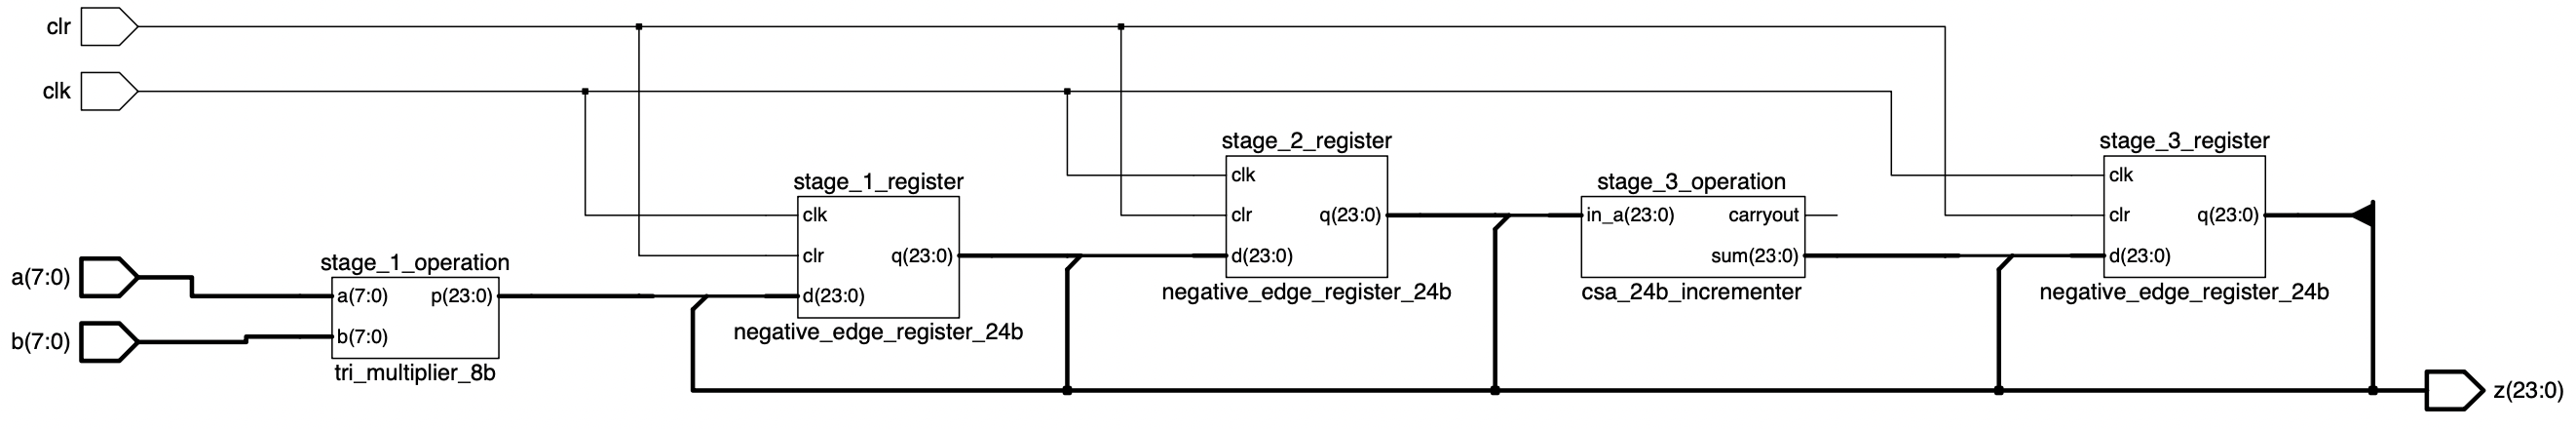
\includegraphics[width=\textwidth]{./img/p_8_op_rtl.png}}
	\label{fig:p_8_rtl}
\end{figure}

\subsection{8-bit Operands Implementation with Output Separation Overflow Handling}

With separation overflow handling discussed before, the full result can be obtained after three stages of calculation with two overflow handling stages.
Before the full data reach the \(Z\) port, the 24-bit result will be separated into 2 parts: the higher part stored in one register and the lower part stored in another register.
The handler takes those two data and transfers them to \(Z\) port alternately by the clock.

\tbref{tb:pip_sep_vi} presents how the z will take over the data and \figref{fig:p_8_sep_sim} shows the simulation of the design.
\figref{fig:p_8_sep_rtl} presents the RTL description of the decign.

\clearpage

\begin{table}[!ht]
	\renewcommand{\arraystretch}{0.8}
	\caption{A Visual Representation Table of the Pipelined Processing with Output Separation Overflow Handling}
	\centering
	\begin{tabular}{ >{\centering\arraybackslash}p{0.5cm} >{\centering\arraybackslash}p{5cm} >{\centering\arraybackslash}p{2.8cm}  >{\centering\arraybackslash}p{2.8cm} >{\centering\arraybackslash}p{2.8cm} }
		\hline
		\bfseries clk & \bfseries Stage 3 Reg    & \bfseries Stage 4 Reg for Higher & \bfseries Stage 4 Reg for Lower & \bfseries Z      \\
		\hline
		...           &                          &                                  &                                 &                  \\
		3             & 000110110000110100101101 & -                                & -                               & -                \\
		4             & -                        & 1000000000110110                 & 0000110100101101                & 1000000000110110 \\
		6             & -                        & 1000000000110110                 & 0000110100101101                & 0000110100101101 \\
		\hline
	\end{tabular}
	\label{tb:pip_sep_vi}
\end{table}

\begin{figure}[!ht]
	\centering
	\caption{Simulation Wave Diagram of the 8-bit Pipelined ALU Circuit with Separation Output}
	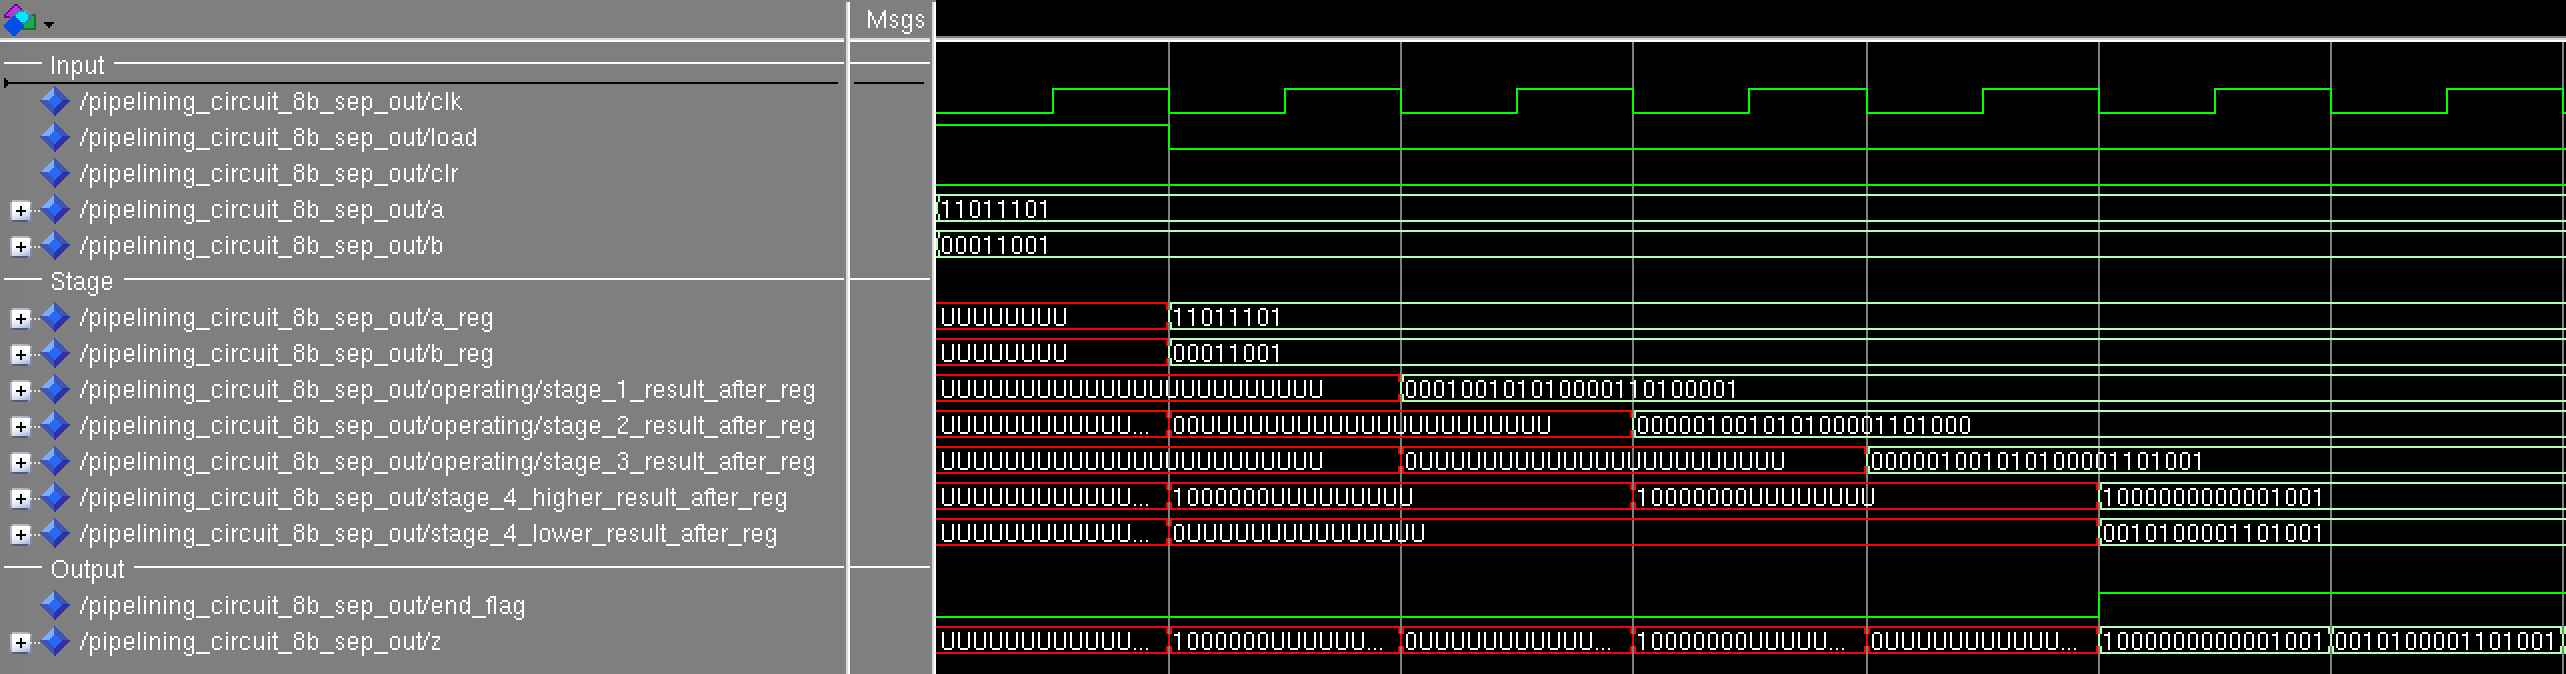
\includegraphics[width=\textwidth]{../img/p_8_sep_sim.png}
	\label{fig:p_8_sep_sim}
\end{figure}

\begin{figure}[!ht]
	\centering
	\caption{Synthesized Diagram of the 8-bit Pipelined ALU Circuit with Separation Output}
	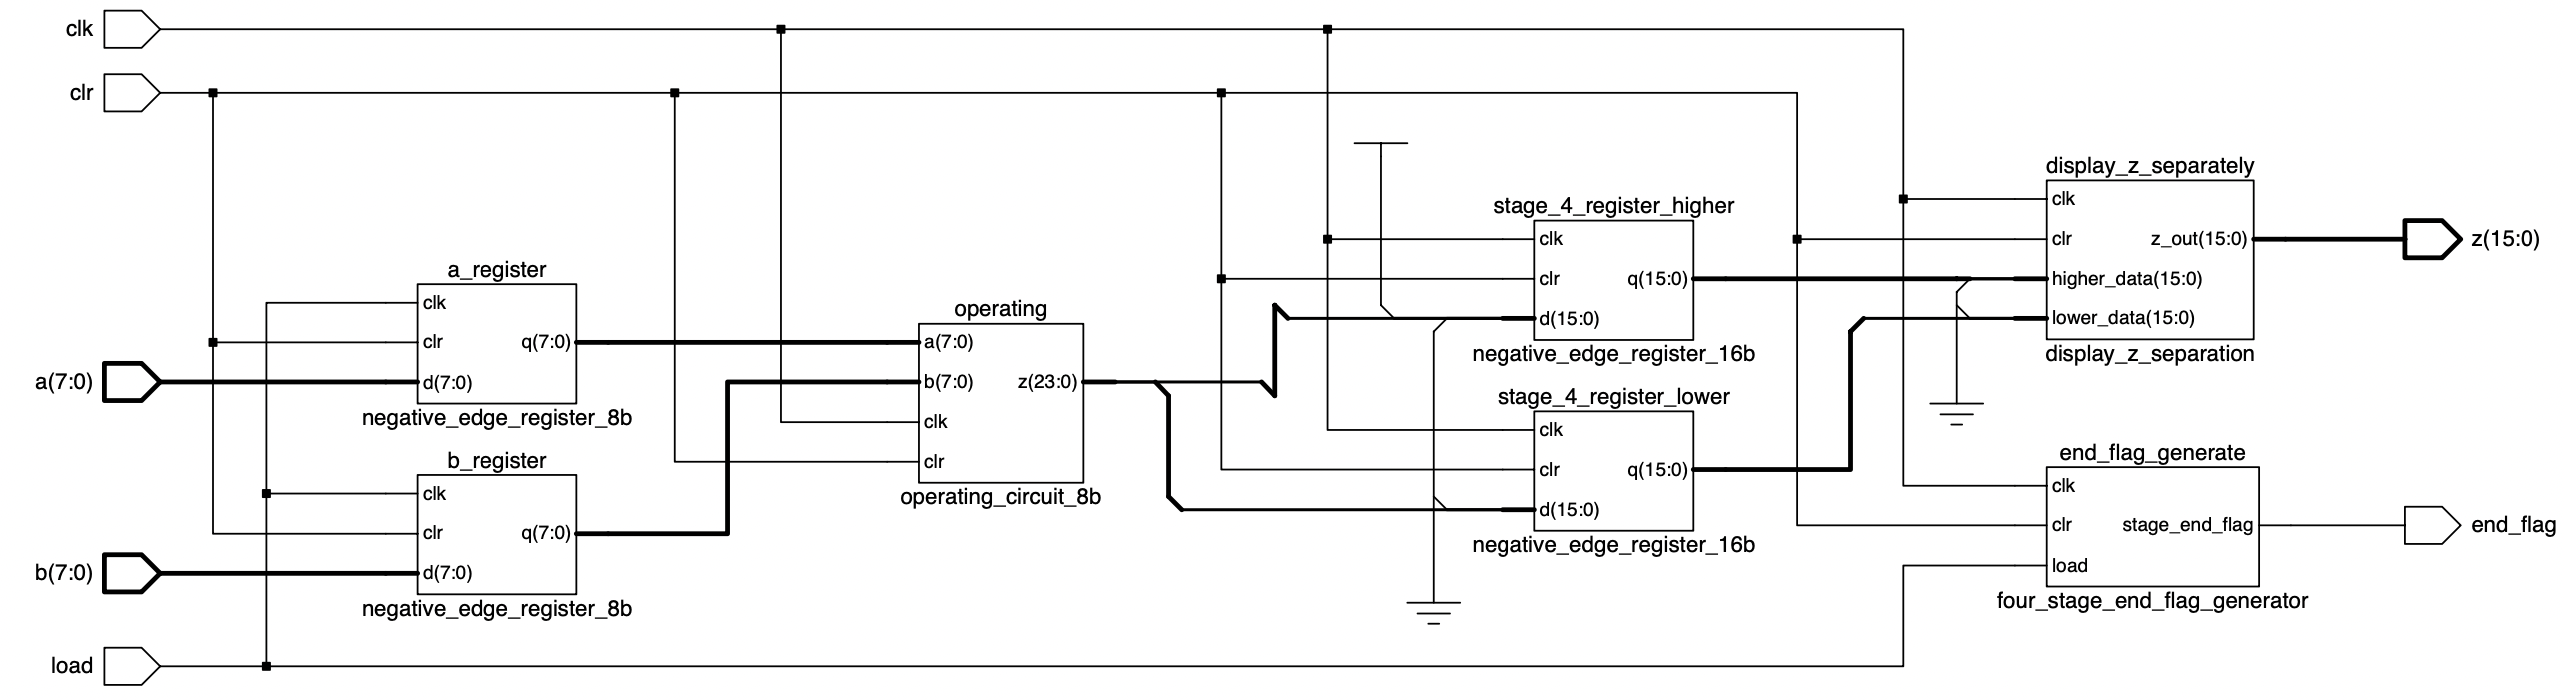
\includegraphics[width=\textwidth]{../img/p_8_sep_rtl.png}
	\label{fig:p_8_sep_rtl}
\end{figure}

\newpage

\subsection{16-bit Operands Implementation and Simulation}

By now there will no necessary for discussing the implementation of the extended design
since all details were presented in the previous sections.
\figref{fig:p_16_sim} presents the testbench simulation of the bit-width extended circuit.


\begin{figure}[!ht]
	\centering
	\caption{Simulation Wave Diagram of the 16-bit Pipelined ALU Circuit with Negation Output}
	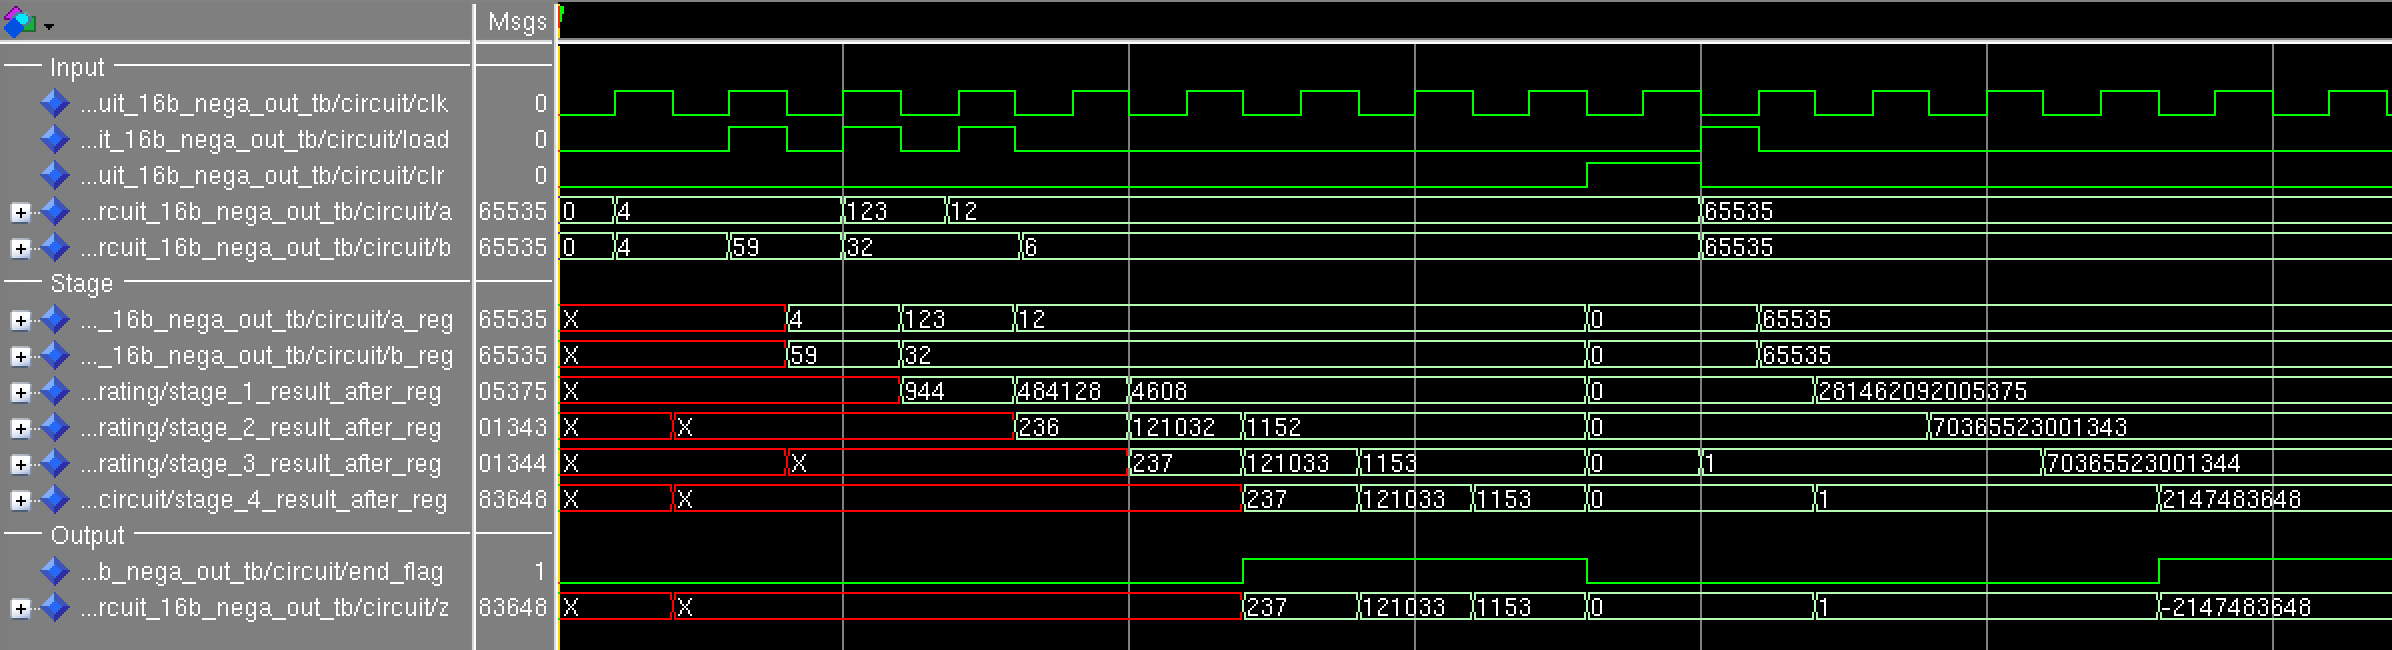
\includegraphics[width=\textwidth]{../img/p_16_sim.png}
	\label{fig:p_16_sim}
\end{figure}